\section{Satellite design planning}
Interdepency relationships among tasks, human resources and level of effort

\begin{longtable}{ | p{1.3cm} | p{7cm} | p{3cm} | p{3.5cm} |}
	\hline
	
	\textbf{ID }& \textbf{Work Package} & \textbf{Time (h)} & \textbf{Prelations} \\ \hline
	\multicolumn{4}{|c|}{\textbf{1. Preliminary design}} \\ \hline
	1. & Preliminary design & 30 &   \\ \hline
	\multicolumn{4}{|c|}{\textbf{2. Structure and mechanics}} \\ \hline
	2.1 & Structure & 6 & BF - 1 \\ \hline
	2.2. & Deployments & 6 & BF - 2.1.  \\ \hline
	2.3. & Thermal protection & 9 & BF - 2.2. \\ \hline
	2.4. & Commercial availability & 12 & BF - 2.3. \\ \hline
	2.5. & Choose option & 6 & BF - 2.4. \\ \hline
	\multicolumn{4}{|c|}{\textbf{3. Electrical Power System}} \\ \hline
	3.1. & Solar arrays & 9 & BF - 1, BB - 5, 6 \\ \hline
	3.2. & Batteries & 9 &BF - 1, BB - 5, 6 \\ \hline
	3.3. & Power management & 12 & BF - 3.1, 3.2\\ \hline
	3.4. & Commercial availability & 15 & BF - 3.3.\\ \hline
	3.5. & Choose option & 9 & BF - 3.4.\\ \hline
	\multicolumn{4}{|c|}{\textbf{4. Propulsion Systems}} \\ \hline
	4.1 & Motivations & 12 & BF - 1, BB - 2  \\ \hline
	4.2 & Commercial availability & 15 & BF - 5  \\ \hline
	4.3 & Choose option & 9 &   BF - 4.2. \\ \hline
	\multicolumn{4}{|c|}{\textbf{5. Payloads}} \\ \hline
	5.1.1. & Data Handling Systems & 15 & BF - 1 \\ \hline
	5.1.2. & Antenna & 12 & BF - 1, FF - 5.1.1. \\ \hline
	5.2. & Commercial availability & 15 & BF - 5.1.  \\ \hline
	5.3. & Choose option & 15 & BF - 5.2.\\ \hline
	\multicolumn{4}{|c|}{\textbf{6. AOCS}} \\ \hline
	6.1. & Attitude determination& 9 & BF - 1, BB - 2  \\ \hline
	6.2. & Attitude control & 9 & BF - 1, BB - 2\\ \hline
	6.3. & Orbital Control & 12 & BF - 1, BB - 4 \\ \hline
	6.4. & Commercial availability  & 20 & BF - 5 \\ \hline
	6.5. & Choose option & 4 &  BF - 6.4.\\ \hline
	\caption{Prelations and Time} \\
\end{longtable}

\section{Gantt of the section}
%\newgeometry{left=0.1cm,bottom=0.1cm}
%\begin{figure}[h]
%\centering
%\includegraphics[width=20cm, height=21cm]{./external_pdf/wbs_final.pdf}
%\end{figure}
\begin{landscape}
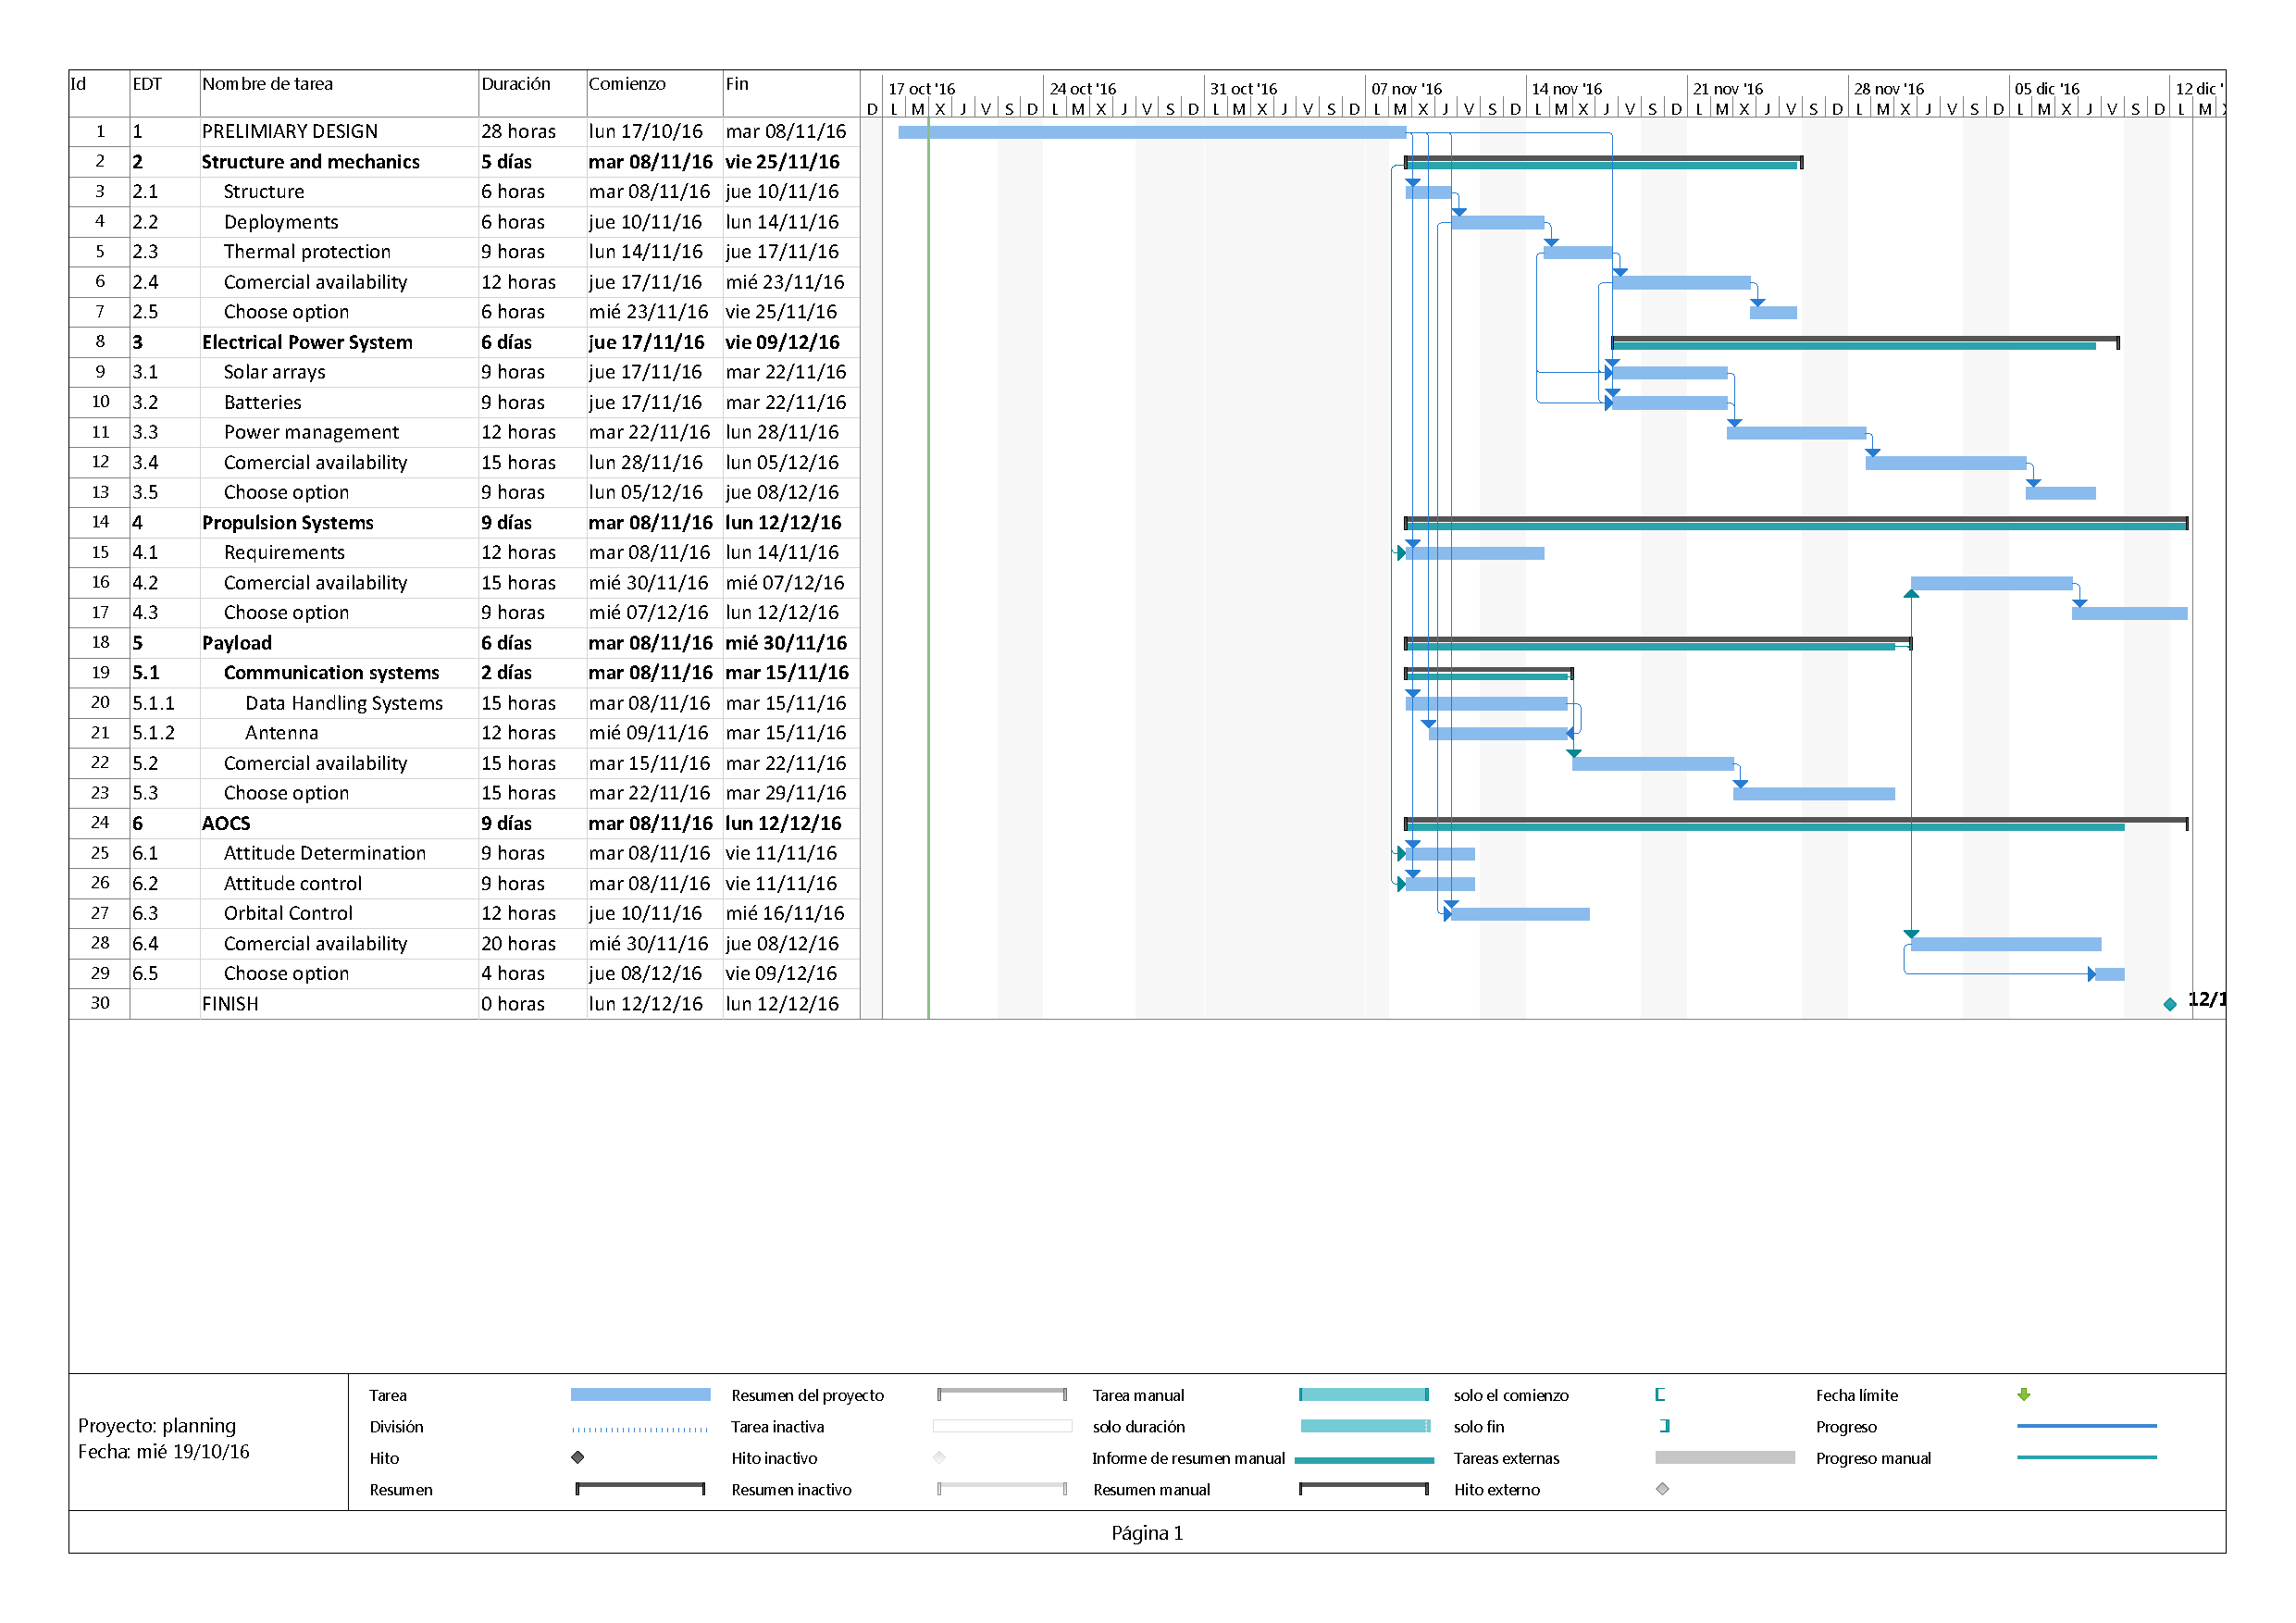
\includepdf[pages={1-}, landscape=true]{./sections/0_Example/GANTT_satellite_design.pdf}
\end{landscape}
%\restoregeometry

